\chapter{Searching for SUSY with $\alpha_{T}$}


The data collected by the CMS detector could hold signs of physics Beyond the Standard Model (BSM). In order to search for signs of new physics they must be distinguished from the vast quantity of Standard Model processes that will arise. Due to the nature of hadron collisions, a large background from QCD events is present, which poses challenges unlike the clean lepton colliders. The events one wishes to look for are termed ``signal" events, and all others become part of the ``background". Search strategies are developed to optimise the selection of desired events whilst rejecting a large proportion of the unwanted ``background" events. The validity of a search is tested using Monte Carlo simulations of both possible signal and expected background events, and is often evaluated by the proportion of signal S to background B, the S/B of a search. 

This thesis focuses on searching for new physics inspired by almost all SUSY models. In this chapter we explore the nature of such new physics and the development of a new variable \alt which forms the backbone of a search for events with quarks and a large quantity of missing energy. 

\section{Inclusive SUSY Search}

As previously discussed in Chapter \ref{ch:theory}, SUSY models that conserve R-Parity and therefore indicate new physics at the TeV scale introduce a candidate particle for dark matter. As this LSP cannot be observed due to its weakly interacting nature, searching for it is analogous to a search for large missing energy in particle collisions. In the CMS detector reconstruction of all visible particles allows us to calculate the transverse component of this quantity, missing $E_{T}$ or \met. 

As there are many models to describe the exact nature of SUSY due to the unknown mechanism of SUSY breaking, it is desirable to design an experimental search which does not rely on any one in particular, or even on the assumption of SUSY. These are called ``inclusive" searches, and retain sensitivity to any new physics resulting in a new particle with the properties of a WIMP. The main feature is a requirement of a large quantity of \met along with final state objects (hadronic jets, leptons, photons). The search space is then divided into channels via the final state objects required, in order to perform orthogonal searches to increase sensitivity and to allow combination 

Discussion of SUSY on the whole and specific models such as mSUGRA are then used to quantify the reach of the search and to tune the cuts with Monte Carlo data. Where no new physics is found it can be useful to set limits on the parameters of such models, and in this thesis we will use mSUGRA for this purpose, along with test points in the mSUGRA phase space. However it is important to remember that the search itself remains open and sensitive to any WIMP candidate. 

Physics at the LHC will suffer from high background rates, especially those from QCD, and the main goal of any analysis is selecting the new physics events required whilst removing the background from Standard Model processes. Missing energy can be observed in events in two ways, real missing energy from the production of weakly interacting particles, such as neutrinos and LSP's, and fake missing energy which is a result of mismeasurment of objects, or missed objects. 

Having noted that the generic signal produced by any such new physics model is a large amount of \met, it might be assumed this forms the main variable to separate signal from background events. As \met is measured in the calorimeters, it can be affected by miscalibration and noise in the detector, thus is not robust for early physics at the LHC. 

To combat this issue there is also the quantity \mht which represents the vector sum of transverse momenta $p_{T}$ of the jets in the system, giving the hadronic missing energy analogous to \met in a hadronic search. However, there are limitations to the use of either of these quantities, as they are not robust to mismeasurments of the jets. 

A background event with no missing energy may therefore be selected as having considerable \met or \mht due to these mismeasurments, and thus it is natural to look for other variables which have a higher discriminatory power. 







\section{$\alpha_{T}$ in a di-jet system}

The first step in devising a SUSY search strategy begins with the simplest of channels, the ``dijet" search with just two jets and missing energy corresponding to two missing neutralinos.  This channel is motivated by one of the cinematic scenarios of mSUGRA mentioned in Chapter \ref{ch:theory}, where the gluino is heavier than the squarks, therefore squarks are liable to decay directly to the LSP producing a quark jet. Due to the low multiplicity it is easy to understand kinematically the situation in play. 

At the LHC the dominant background is from QCD diet events, produced with an extremely large cross section. These events do not actually produce \met but can ``fake" this signature through detector effects such as mismeasurment or missed objects. In addition there are a number of other backgrounds from electroweak interactions, W + jets, $t \bar{t}$ and Z $\rightarrow \nu \bar{\nu}$ + jets, which we will refer to collectively as EWK. Due to the ``fake" \met signature from QCD events, a significant proportion of these events are not eliminated by a simple \met or \mht cut. 

In a QCD diet event, were it to be perfectly measured, the two jets are pair produced and following conservation laws must be back-to-back and of equal magnitude. In events with real missing energy, such as our potential SUSY signal, the jets have been produced independently of one another, and such rules do not govern them. The distribution of the azimuthal angle between the two jets, $\Delta \phi$, is therefore very different for the QCD background and potential signal events, shown in Figure XX. 


It is possible to exploit the nature of this further using a new variable proposed by Randall and Tucker-Smith, $\alpha$, defined in Equation \ref{eqn:alpha}~\cite{Randall}. 

\begin{equation}
\alpha = \frac{E_{T}^{j2}}{M_{inv}^{j1,j2}}
\label{eqn:alpha}
\end{equation}

The $E_{T}^{j2}$ is the transverse energy of the second jet (the lowest in energy) and $M_{inv}^{j1,j2}$ is the invariant mass of the dijet system. The design of this variable allows us to exploit the expected back-to-back nature of any dijet from QCD. A well-measured QCD event can only take values of $\alpha < 0.5$. In sharp contrast, a SUSY event can, due to the unseen neutralinos, produce jets in a similar direction with a low invariant mass giving rise to high values of $\alpha$.

The transverse variant of this variable, given in Equation \ref{eqn:alpha} makes use of the transverse mass $M_{T}$ of the two jets as opposed to the invariant mass.

\begin{equation}
\alpha_{T} = \frac{E_{T}^{j2}}{M_{T}} 
\label{eqn:alphat}
\end{equation}

In this case a well-measured QCD event will have exactly 0.5. While both show equally strong power of background discrimination, $\alpha_{T}$ has greater signal retention for certain mSUGRA points,\cite{PASaT} and therefore is deemed comparable or superior. It is upon this variable that the search strategy is formed. The presence of the second jet energy in the numerator also gives rise to one of the most important properties of this variable, its resilience to jet mismeasurment. If there is a large mismeasurment of one of the jets, the order could be inverted. As a perfectly measured QCD event yields \alt = 0.5, the cut chosen is \alt > 0.55 in order to take into account the finite resolution of the jet energy measurement.  


The explicit reliance of \alt on $\Delta \phi$ can be seen when the relationship is rewritten in the massless limit, in Equation \ref{eqn:alphatphi}. This relationship indicates a high correlation, and thus a cut on \alt renders a further cut on $\Delta \phi$ negligible\cite{ANaT}.

\begin{equation}
\alpha_{T} = \frac{\sqrt{E_{T}^{j2}/E_{T}^{j1}}}{2(1- \textrm{cos} \Delta \phi)} 
\label{eqn:alphat}
\end{equation}


\section{$\alpha_{T}$ in a n-jet system}
More complicated decay processes result in hadronic signatures with more than two jets, generalised to the n-jet system, for example where a gluino-squark pair decay to produce three quarks and two LSP's. In order to increase phase space the dijet search channel may be extended to a final state including N jets and considerable \met, where N $\geq$ 2. This is colloquially known as the all-hadronic search channel as it comprises any fully-hadronic decay modes that might yield possible SUSY signal. 

Following the success of the construction of the \alt variable in the dijet topology, the variable was extended to a general form applicable for an n-jet system, thus incorporating the full hadronic SUSY search channel\cite{ANnaT} . This is undertaken by modelling the system of $n$ jets as though it were a diet system, through the mathematical construction of two pseudo jets. Thus \alt can be calculated using the properties of the pseudo jets. 

The two pseudo-jets are built by merging the n jets present in two sets with a vectorial sum deciding the direction, and a length equal to the sum of the magnitudes of the composite jets. The combinations chosen to assign n jets into 2 pseudo jets is done such that they are as balanced as possible, i.e. the difference in \HT, $\Delta \HT$ is at a minimum. All combinations are therefore considered, and the one which satisfies this condition is chosen. With this psedo-dijet system we can construct a formalism for \alt that uses the basic kinematic variables of the system in Equation \ref{alphat_njet}. 

\begin{equation}
\alpha_{T} =\frac{1}{2} \frac{(\HT - \Delta \HT)}{\sqrt{\HT^{2} - |\mht|^{2}}}  = \frac{1}{2} \frac{1-\Delta \HT / \HT}{\sqrt{1 - (\mht / \HT)^{2}}}
\label{eqn:alphat_njet}
\end{equation}

The second form of the definition shows its dependence on the ratios of $\Delta \HT$ and \mht to the events \HT. In a well measured QCD event there is no \mht, and $\Delta \HT / \HT < \sfrac{1}{3}$, from which the maximal value comes from the rare ``Mercedes Star" QCD event with three jets of equal mass and momenta with the $\Delta \phi$ between any chosen two being equal. Therefore with an ideal detector QCD events have $0.333 < \alt < 0.5$, but large mismeasurment leads to a high \mht which can higher the values of \alt. The chosen cut value of \alt $>$ 0.55 corresponds to a missing energy fraction \mht / \HT $>$ 0.4, and as this occurs in QCD events the ratio $\Delta \HT / \HT$ is liable to increase also. This relationship prevents \alt for QCD events from significantly exceeding 0.5 unless an object of sizeable momentum were missed altogether in the calculation. 

It has been shown that whilst the sharp cut-off for QCD events at \alt = 0.5 becomes less distinct, it is still pronounced and thus retains the powerful background rejection properties desired\cite{an2009_56}. Performance tests with smeared jet energies shows the \alt variable applied to a multi-jet analysis is robust to jet mismeasurment, and superior in this area to a standard \met analysis. The jet energy scale does not directly affect \alt but its resolution improves for increasing \HT, as demonstrated with 7 TeV data in Reference \cite{an2010_119}. 

\section{Defining the ratio \RaT}

The proportion of SUSY signal to background differs greatly with the \HT of the event, with background processes dominating at low values while SUSY becomes more prominent for high \HT. In order to investigate this behaviour a new variable \RaT is defined in Equation \ref{eqn:rat} as the ratio of events passing the \alt cut with those that fail it. 

\begin{equation}
\RaT = \frac{N(\alt > 0.55)}{N(\alt < 0.55)}
\label{eqn:rat}
\end{equation}

The relationship of this variable with \HT that can then be studied for background processes and potential SUSY signal using Monte Carlo samples. Where QCD events with no real missing energy dominate the numerator, tightening the \HT cut results in a decreasing \RaT. If the QCD background is negligible due to a successful \alt cut, the now-dominating  electroweak backgrounds contribute some real missing energy in the form of neutrinos and exhibit a flat relationship with \HT. However, in the presence of an mSUGRA SUSY signal in the numerator an increase of \HT corresponds to an increasing \RaT. These three distinctive behaviours provide a strong search strategy using \RaT in exclusive bins of \HT. These trends have been shown to be robust to jet mismeasurments, or even when 1 jet in 25 is not included in the calculation \cite{}



\section{Extending \alt for single-lepton searches}

A cleaner SUSY signature can be obtained through the single lepton channel, where the kinematics are identical save the extra requirement that there be one muon or electron in the final state. In addition, requiring a lepton can provide a useful control sample for the hadronic search. Hence it is interesting to develop the \alt search to apply to this channel, especially where the lepton $p_{T}$ is low and hence the dominant background is from fake leptons in QCD events. 

In this case, in the final state there is one lepton, and n jets where n is at least two. Production mechanisms for one lepton and two jets in SUSY decay modes at the LHC are similar to those of the 3-jet hadronic channel. Thus it is possible to draw parallels, and describe the system as an n-object system. Here, an n-jet hadronic event is treated the same as that which has 1 lepton and n-1 jets.  The quantities in the definition of \alt are extended to include the lepton as if it were a jet, such that the lepton is included in the building of the two pseudo-jets. 

The validity of this approach can be seen in Figure \ref{fig:aTnobj} where the hadronic (0-lepton) and single leptonic (1-lepton) cases are shown superimposed for the SUSY test point LM0, for three different object multiplicities 3, 4 and 5. As can be seen, although the shape of the /alt distributions change with the object multiplicity, there is a good agreement between the n jet system and the n-1 jet plus lepton system. 

\begin{figure}
\centering
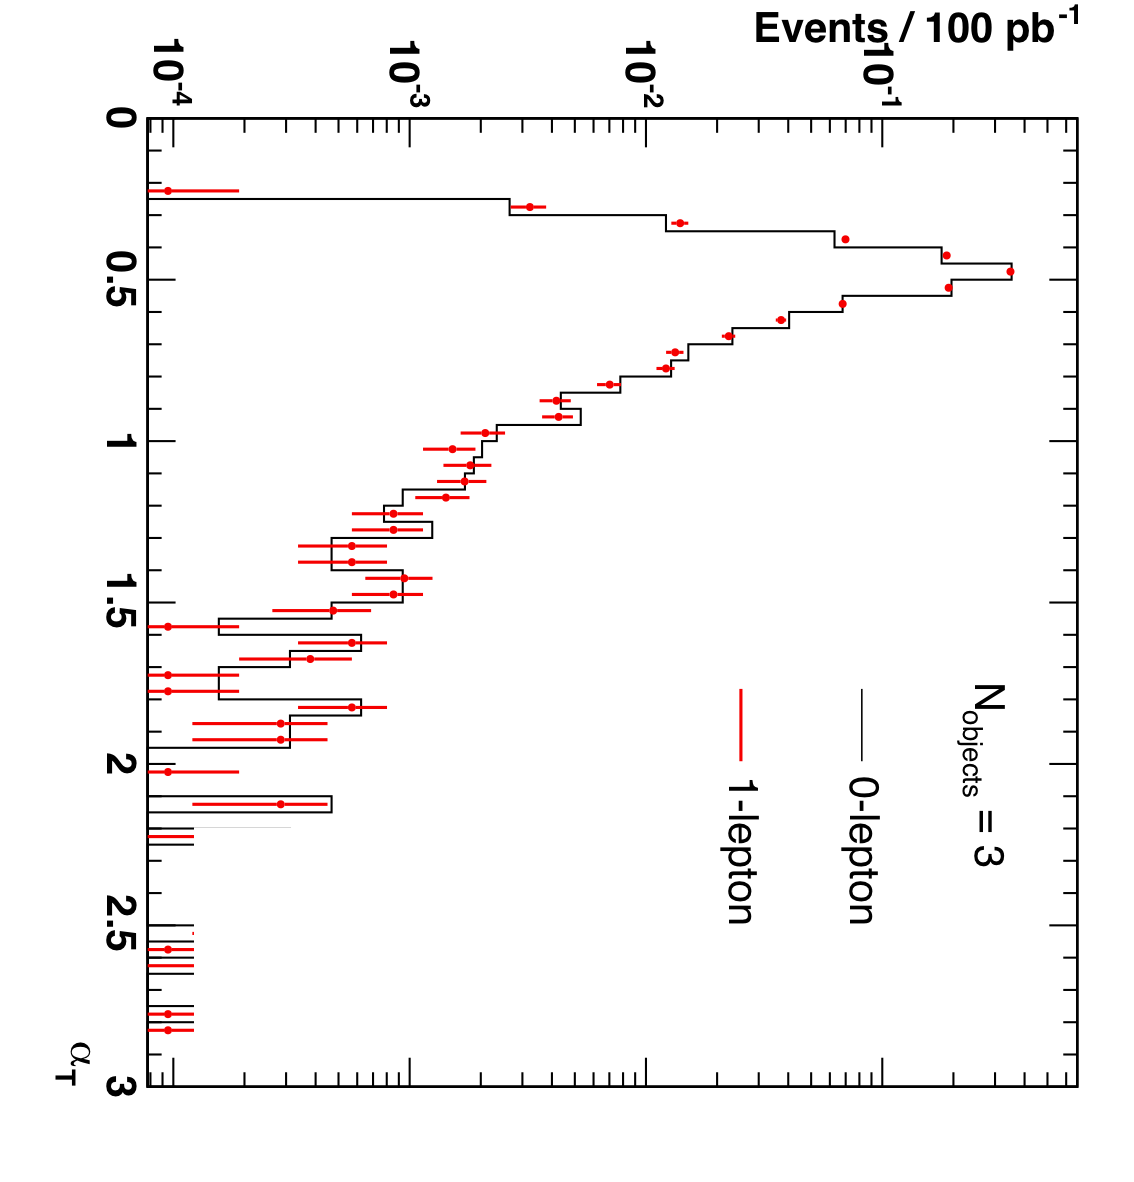
\includegraphics[width=0.3\textwidth, angle=90]{Figures/AlphaT/aT_3}
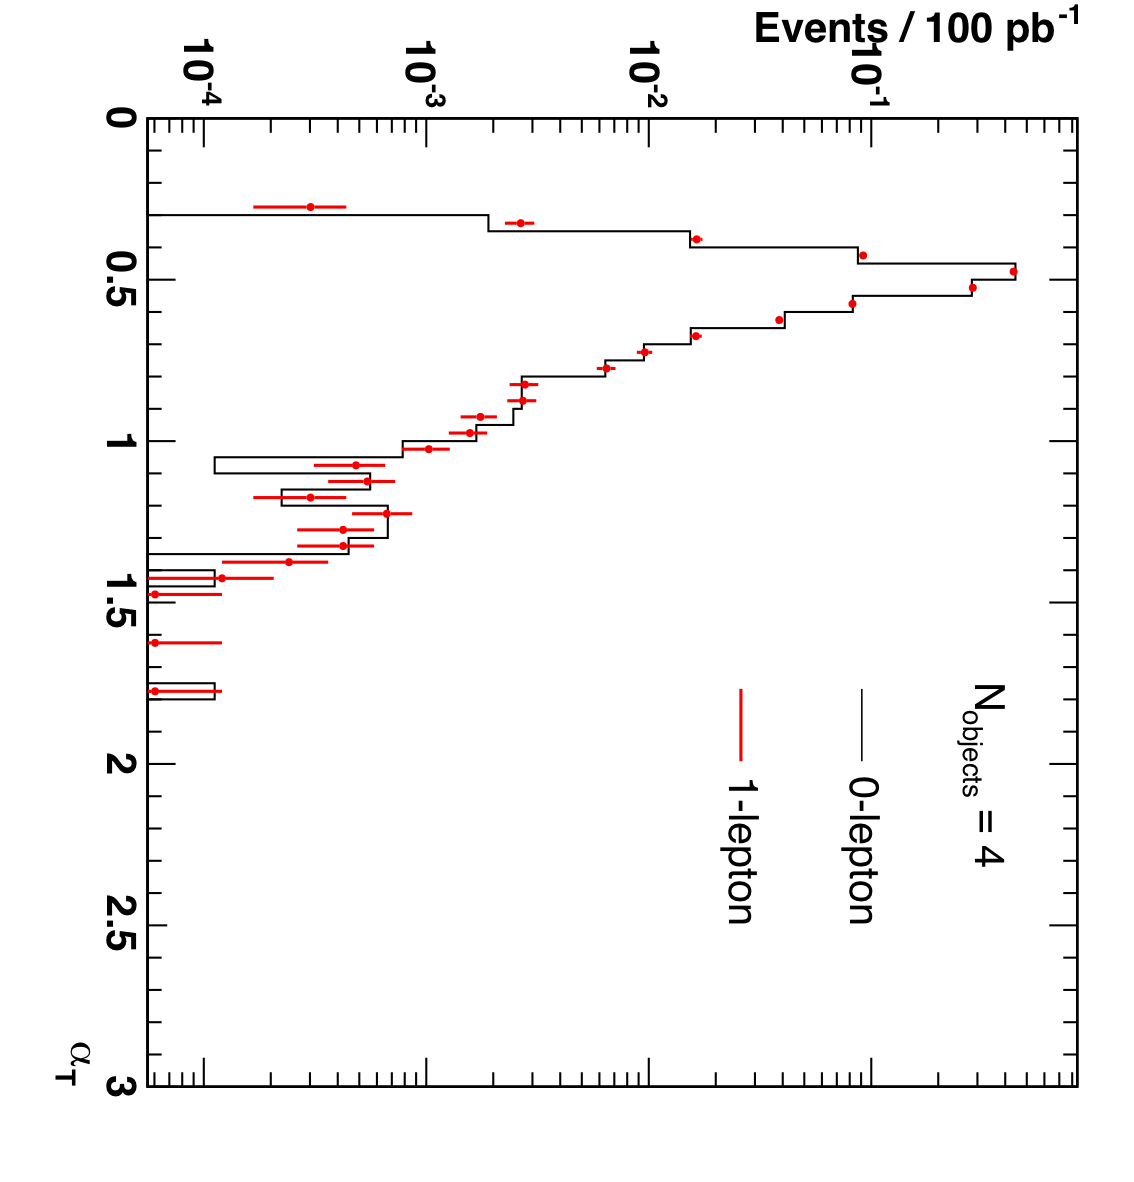
\includegraphics[width=0.3\textwidth,angle=90]{Figures/AlphaT/aT_4}
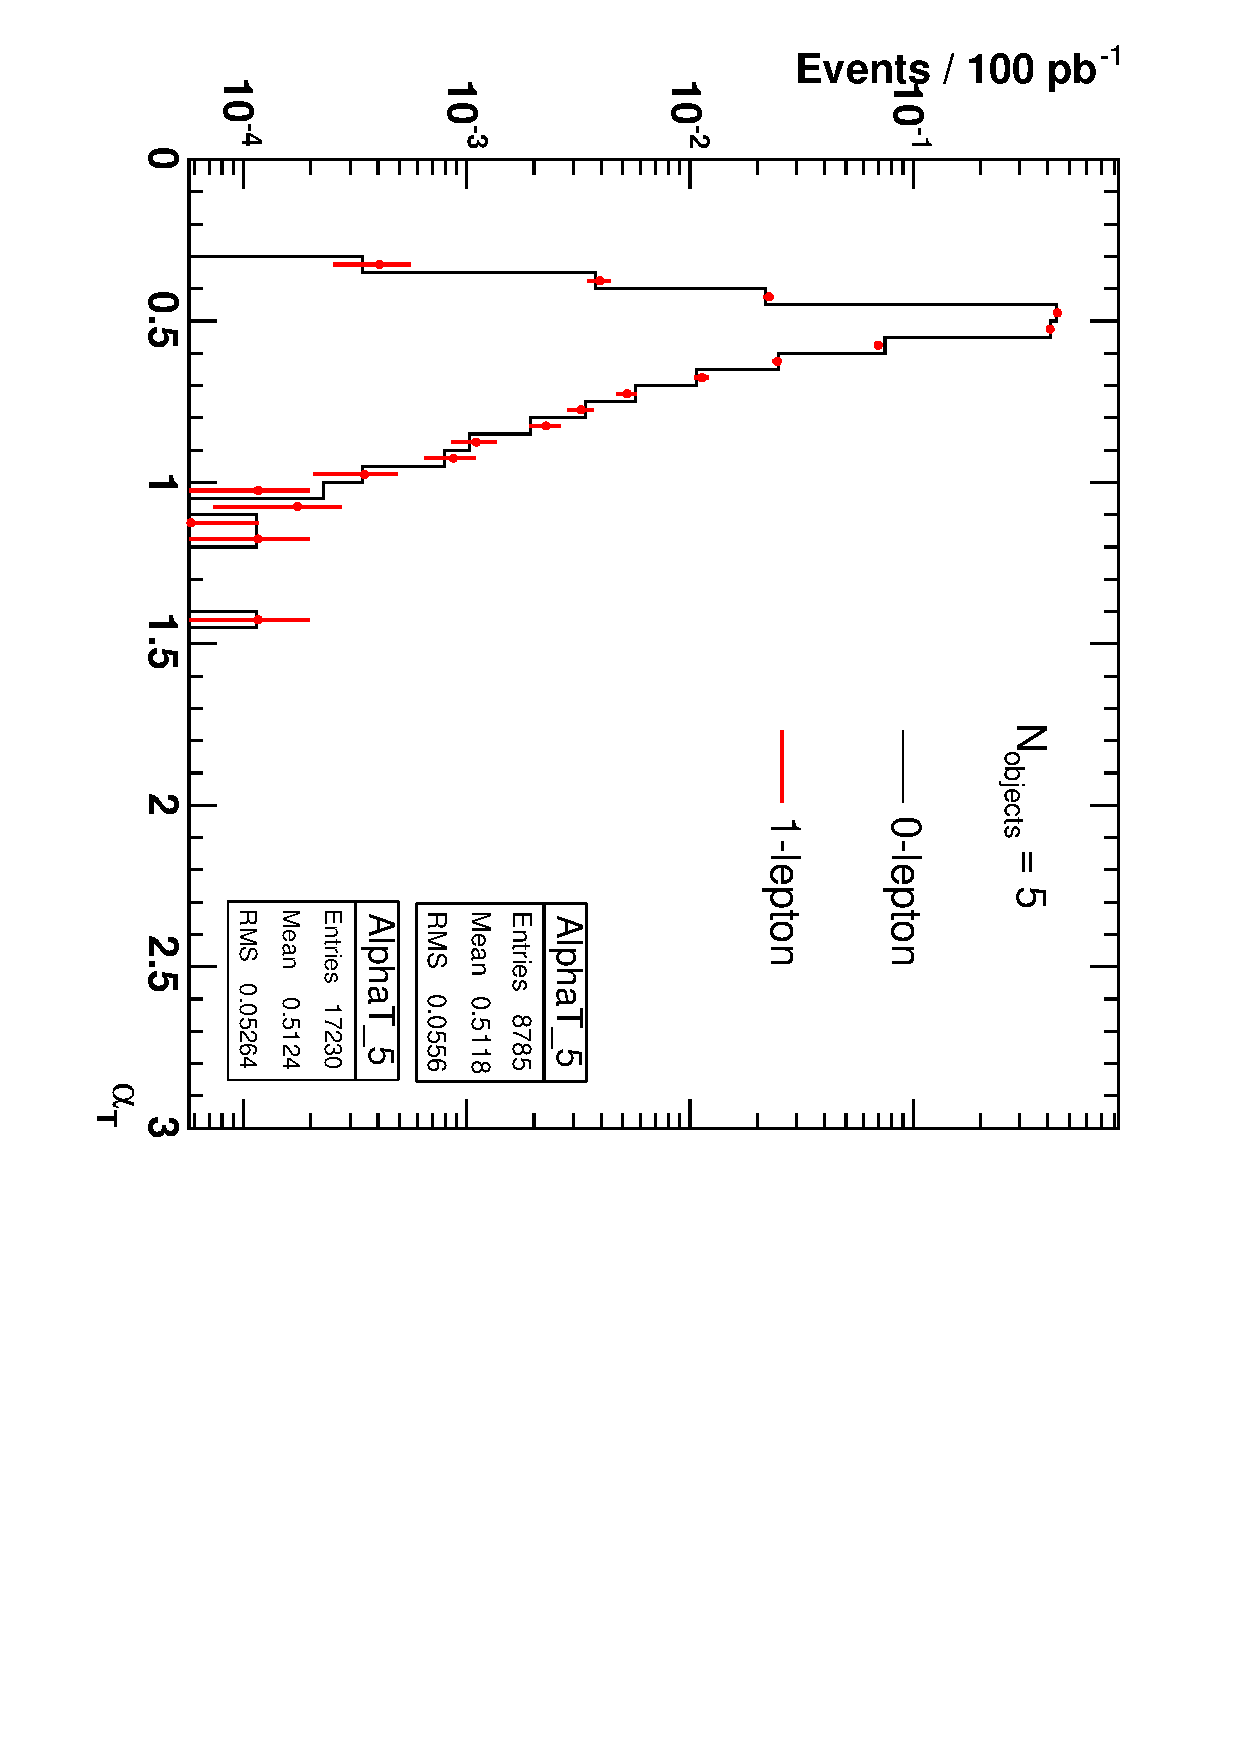
\includegraphics[width=0.3\textwidth,angle=90]{Figures/AlphaT/aT_5}
\caption{\label{fig:aTnobj}The shape of the \alt distributions for object multiplicity N for the N-jet channel (0-lepton) and the N-1 jet plus 1 lepton channel superimposed. From left to right the object multiplicities shown are N=3, N=4, N=5.}
\end{figure}

\section{Reliance of \alt on jet object definition}

As mentioned above, although \alt is robust to mismeasurments a large value can be obtained from a QCD event if significant objects are not included in the measurement. To remain within the capabilities of the detector and reconstruction algorithms, the definition of a jet for the purpose of analysis requires the passing of a certain jet energy threshold. As this value is relatively small compared to the total \HT of an event, it should not contribute a large mismeasurment effect to the \alt variable. However there might be some cases for high jet multiplicities where a large number of low-energy jets just below the threshold are not considered, and so the \alt value is skewed. Hence, to remove this effect it is possible to make a cut in the ratio of the missing energy estimated from jets \mht and that measured by the calorimeter systems \met so that an event with $R_{miss} > 1.25$ is rejected. 
